\documentclass[12pt, letterpaper]{article}

%% preamble: Keep it clean; only include those you need
\usepackage{amsmath}
\usepackage[margin = 1in]{geometry}
\usepackage{graphicx}
\usepackage{pgfplots}
\usepackage{booktabs}
\pgfplotsset{compat=1.18, width=10cm}
\usepackage{natbib}

% for space filling
\usepackage{lipsum}
% highlighting hyper links
\usepackage[colorlinks=true, citecolor=blue]{hyperref}

\title{My first LaTeX document}
\author{Richa Patel}
\date{September 25, 2023}

\begin{document}

\maketitle 

\begin{abstract}
The goal of the Paper is to use to our first \LaTeX{} document! and create a new Manuscript.
\end{abstract}

\section{Introduction}
\label{sec:intro}

The following is the background of this topic.

%roadmap
The restof the paper is organized as follows:
The data are presented in Section~\ref{sec:data}
The tables are presented in Scetion~\ref{sec:tab}
the Methods are presented in Section~\ref{sec:meth}
Conclution contains in Section~\ref{sec:con}

\section{Data}
\label{sec:data}

This is the first section.It displays Images

Figure~\ref{fig:Image1} Shows the Scatterplot created

\begin{figure}[tbp]
  \centering
  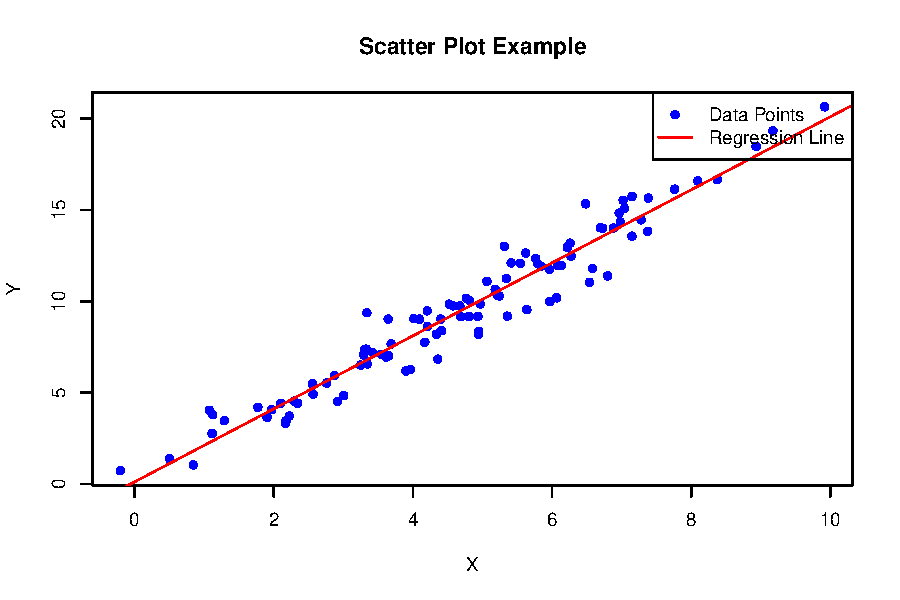
\includegraphics[width=\textwidth]{Image1.pdf}
  \caption{This is my first figure.}
  \label{fig:Image1}
\end{figure}


\section{Tabels}
\label{sec:tab}

It displays table 1.1

\begin{table}[tbp]
\centering
\caption{This is my First Table}
\begin{tabular}{|l|l|}  
\hline
Observation & Distance \\ \hline
1           & 3        \\
2           & 2        \\ 
3           & 3.16     \\ 
4           & 2.24     \\ 
5           & 1.41     \\ 
6           & 1.73     \\ \hline
\end{tabular}
\end{table}

\section{Methods}
\label{sec:meth}


Here f is some fixed but unknown function of X1,...,Xp, and " is a random
error term, which is independent of X and has mean zero. In this formula- error term
tion, f represents the systematic information that X provides about Y. As shown below in the graph 1.2

\subsection{Equations}
This is the first section.It displays Math Equations.

\begin{itemize}

  \item More generally, suppose that we observe a quantitative response Y and p different predictors, X1, X2,...,Xp. We assume that there is some relationship between Y and X = (X1, X2,...,Xp), which can be written in the very general form
  
  \[Y = f(X)+\epsilon\]

  \item Consider a given estimate $\hat{f}$ and a set of predictors X, 
  which yields the prediction $\hat{Y} = \hat{f}(X)$.  Assume for a moment that both $\hat{f}$ and X are fixed,
  so that the only variability comes from ". Then, it is easy to show that

  $E(Y-\hat{Y})^2$=$E[f(X)+\epsilon-f(X)]^2$
  $=\underbrace{[f(X)-\hat{f}(X)]^2}_{Reducible}$+$\underbrace{Var(\epsilon)}_{Irreducible}$
  
\section{Conclusion}
\label{sec:con}

 At the end i would like to conclude that making a Latex document is not easy. especially for a non coder background.
Items that are cited:\cite{latexcompanion} and \cite{LoveJonathon2019JGss}

\end{itemize}

\bibliography{refs}
\bibliographystyle{plain}
\end{document}
